\documentclass{article}


% if you need to pass options to natbib, use, e.g.:
%     \PassOptionsToPackage{numbers, compress}{natbib}
% before loading neurips_2022


% ready for submission


% to compile a preprint version, e.g., for submission to arXiv, add add the
% [preprint] option:
%     \usepackage[preprint]{neurips_2022}


% to compile a camera-ready version, add the [final] option, e.g.:
\usepackage[final]{neurips_2022}
\title{Posthoc Interpretation via Quantization}

% to avoid loading the natbib package, add option nonatbib:
%    \usepackage[nonatbib]{neurips_2022}


\usepackage[utf8]{inputenc} % allow utf-8 input
\usepackage[T1]{fontenc}    % use 8-bit T1 fonts
\usepackage{hyperref}       % hyperlinks
\usepackage{url}            % simple URL typesetting
\usepackage{booktabs}       % professional-quality tables
\usepackage{amsfonts}       % blackboard math symbols
\usepackage{nicefrac}       % compact symbols for 1/2, etc.
\usepackage{microtype}      % microtypography
\usepackage{xcolor}         % colors

\usepackage{microtype}
\usepackage{graphicx}
\usepackage{subfigure}
\usepackage{booktabs} % for professional tables
\usepackage{xparse,xfp}

% hyperref makes hyperlinks in the resulting PDF.
% If your build breaks (sometimes temporarily if a hyperlink spans a page)
% please comment out the following usepackage line and replace
% \usepackage{icml2023} with \usepackage[nohyperref]{icml2023} above.
\usepackage{hyperref}
\usepackage{multirow}

% Attempt to make hyperref and algorithmic work together better:
\newcommand{\theHalgorithm}{\arabic{algorithm}}

% Use the following line for the initial blind version submitted for review:
% If accepted, instead use the following line for the camera-ready submission:
% \usepackage[accepted]{icml2023}

% For theorems and such
\usepackage{amsmath}
\usepackage{amssymb}
\usepackage{mathtools}
\usepackage{amsthm}

% if you use cleveref..
\usepackage[capitalize,noabbrev]{cleveref}
\usepackage{float}
\floatstyle{plain} % optionally change the style of the new float
\newfloat{Code}{H}{myc}


%%%%%%%%%%%%%%%%%%%%%%%%%%%%%%%%
% THEOREMS
%%%%%%%%%%%%%%%%%%%%%%%%%%%%%%%%
\theoremstyle{plain}
\newtheorem{theorem}{Theorem}[section]
\newtheorem{proposition}[theorem]{Proposition}
\newtheorem{lemma}[theorem]{Lemma}
\newtheorem{corollary}[theorem]{Corollary}
\theoremstyle{definition}
\newtheorem{definition}[theorem]{Definition}
\newtheorem{assumption}[theorem]{Assumption}
\theoremstyle{remark}
\newtheorem{remark}[theorem]{Remark}
\usepackage{tikz}
\usetikzlibrary{shapes,arrows,snakes}
\usetikzlibrary{arrows.meta,arrows}
\usepackage{hyperref}
\usepackage{listings}
\usepackage{xcolor}

\definecolor{codegreen}{rgb}{0,0.6,0}
\definecolor{codegray}{rgb}{0.5,0.5,0.5}
\definecolor{codepurple}{rgb}{0.58,0,0.82}
\definecolor{backcolour}{rgb}{0.95,0.95,0.92}

\lstdefinestyle{mystyle}{
    backgroundcolor=\color{backcolour},   
    commentstyle=\color{codegreen},
    keywordstyle=\color{magenta},
    numberstyle=\tiny\color{codegray},
    stringstyle=\color{codepurple},
    basicstyle=\ttfamily\footnotesize,
    breakatwhitespace=false,         
    breaklines=true,                 
    captionpos=b,                    
    keepspaces=true,                 
    % numbers=left,                    
    numbersep=5pt,                  
    showspaces=false,                
    showstringspaces=false,
    showtabs=false,                  
    tabsize=2
}

\lstset{style=mystyle}
\usepackage[textsize=tiny]{todonotes}


\author{%
  Cem Subakan\thanks{Equal Contribution}    $^{1,2,3}$, Francesco Paissan\footnotemark[1]  $^{4}$, Mirco Ravanelli$^{2,3}$ \\
   \\
  $^1$Université Laval, $^2$Concordia University, $^3$Mila, Québec AI Institute, $^4$University of Trento
   \\
}


\begin{document}


\maketitle


% Recommended, but optional, packages for figures and better typesetting:


% The \icmltitle you define below is probably too long as a header.
% Therefore, a short form for the running title is supplied here:
\newcommand{\thetitle}{Posthoc Interpretation via Quantization}
\newcommand{\cem}[1]{\textbf{$\mathcal{CEM}$: #1}}
\newcommand{\franz}[1]{\textbf{$\mathcal{Francesco}$: #1}}


\tikzstyle{specialblock} = [draw, ultra thick, fill=blue!20, rectangle, 
    minimum height=3em, minimum width=4em]
\tikzstyle{block} = [draw, fill=lightgray, rectangle, 
    minimum height=3em, minimum width=4em]
\tikzstyle{sum} = [draw, fill=white, circle, node distance=1cm]
\tikzstyle{prod}   = [circle, minimum width=8pt, draw, inner sep=0pt, path picture={\draw (path picture bounding box.south east) -- (path picture bounding box.north west) (path picture bounding box.south west) -- (path picture bounding box.north east);}]
\tikzstyle{sumt}   = [circle, minimum width=8pt, draw, inner sep=0pt, path picture={\draw (path picture bounding box.east) -- (path picture bounding box.west) (path picture bounding box.south) -- (path picture bounding box.north);}]
\tikzstyle{input} = [coordinate]
\tikzstyle{output} = [coordinate]
\tikzstyle{pinstyle} = [pin edge={to-,thin,black}]
\tikzset{
tmp/.style  = {coordinate}, 
dot/.style = {circle, minimum size=#1,
              inner sep=0pt, outer sep=0pt},
dot/.default = 6pt % size of the circle diameter 
}

% this must go after the closing bracket ] following \twocolumn[ ...

% This command actually creates the footnote in the first column
% listing the affiliations and the copyright notice.
% The command takes one argument, which is text to display at the start of the footnote.
% The \icmlEqualContribution command is standard text for equal contribution.
% Remove it (just {}) if you do not need this facility.

%\printAffiliationsAndNotice{}  % leave blank if no need to mention equal contribution
%\printAffiliationsAndNotice{\icmlEqualContribution} % otherwise use the standard text.

\begin{abstract}
%This document provides a basic paper template and submission guidelines.
%Abstracts must be a single paragraph, ideally between 4--6 sentences long.
%Gross violations will trigger corrections at the camera-ready phase.

% Old version
%In this paper, we propose \emph{PIQ:Posthoc Interpretation via Quantization}, a posthoc method for interpreting classifier decisions. PIQ uses vector quantization to embed the representations of an already trained classifier into a discrete latent space. The discrete latent space enables restricting specific regions in the latent space dedicated to each class. This restriction is used as a bottleneck to force the interpretations to follow the distribution of the class that corresponds to the classifier decision. Through a series of user studies on images and audio, we observe that our method results in interpretations better preferred by humans compared to several different interpretation methods in the literature.  

% Mirco's new version
In this paper, we introduce a new approach, called \emph{Posthoc Interpretation via Quantization (PIQ)}, for interpreting decisions made by trained classifiers. Our method utilizes vector quantization to transform the representations of a classifier into a discrete, class-specific latent space. The class-specific codebooks act as a bottleneck that forces the interpreter to focus on the parts of the input data deemed relevant by the classifier for making a prediction. We evaluated our method through quantitative and qualitative studies and found that PIQ generates interpretations that are more easily understood by participants to our user studies when compared to several other interpretation methods in the literature.

%reconstructions when tested on overlapped digit classification, and sound event classification.  
% we eventually need to be more specific here
\end{abstract}

\section{Introduction}

% Mirco's first two paragraphs
Deep neural networks have shown remarkable performance in various classification tasks, but they often remain opaque, making it hard for humans to comprehend how they make decisions. Interpretability is the ability to understand and explain a model's predictions. This desirable property is particularly valuable in areas such as healthcare, where collaboration and mutual understanding between humans and AI systems are crucial.

This paper proposes a method for interpreting neural network decisions by reconstructing relevant parts of the input data through vector quantization. This approach is a step towards achieving the ``understandability'' principle outlined in \cite{gilpin2018}, which aims to answer the question, ``\textit{Why does this particular input lead to that particular output?}''. Our goal is to provide clear, human-understandable explanations for neural network decisions, highlighting the specific parts of the input that influence the outcome.
%Deep neural networks yield impressive performance on a variety of classification tasks, but mainly remain black-box models that are hard to explain and interpret. In this paper, we introduce a neural network interpretation method, which aims to explain why a classifier makes its decision by highlighting the relevant portions of the input data.
%reconstructs the data to explain why a neural network classifier makes its decision. 
%In other words, our goal is to provide a reconstruction of the input data, in the same domain to present the user with an explanation for the neural network decision. This is in line with the understandability criterion described in \cite{gilpin2018}: We would like to answer the question, \emph{Why does this particular input lead to that particular output?} In our view, the neural network interpretations should be easy to understand by humans and should explain the parts of the input which cause the neural network to make its decision. 
% Mirco's version (minor changes):

In Figure \ref{fig:introshowcase}, we show a use-case of neural network interpretations. The left panel shows overlapping digits from the MNIST dataset \cite{lecun-mnisthandwrittendigit-2010}. 
As can be observed, it is hard to discern the dominant digit. To gain insight into how the neural network makes its decision, it would be useful to identify which parts of the image it focuses on. The right panel shows the output of our method as red overlays applied on top of the mixtures. We can see that the explanations provided by PIQ emphasise the parts of the input that correspond to the classifier's decisions (shown in green text). Additionally, our approach can be straightforwardly applied to audio as well, with examples available on our companion website\footnote{\url{https://piqinter.github.io/}}.

%In Figure \ref{fig:introshowcase}, we show a use-case of neural network interpretations. Namely, on the left panel we have overlapping digits from the MNIST dataset \cite{lecun-mnisthandwrittendigit-2010}. As can be seen, in some cases it is hard to decide which is the more dominant digit, and therefore it would be useful to understand which parts of the image the neural network pays attention to make its decision. On the right panel, we show the output of our method with red overlays. We see that the explanations provided by our method outline the parts of the input which correspond to the classifier decisions (shown with green text overlay) on the top right corner of each digit. Similarly, our method applies to audio as well, and example interpretations are provided on our \href{https://piqinter.github.io/}{companion website}. 

\begin{figure}
    \centering
    \includegraphics[width=.235\textwidth]{mnistmixtures/samples_1.png}
    \includegraphics[width=.235\textwidth]{mnistmixtures/superpose_ours_1.png}
    \caption{Showcasing the classifier interpretations generated by PIQ. The \textbf{(left)} panel displays the input images, with the classifier's decisions marked in green. On the \textbf{(right)}  panel, the PIQ interpretations are highlighted in red on the original image.}
    \label{fig:introshowcase}
\end{figure}

% Mirco's version (minor changes)
 To accomplish this, PIQ learns specific latent representations for each class. In particular, we embed the classifier's latent representations into a discrete latent space that is compartmentalized according to the classes available in the training dataset. We use the vector quantization objective, which was first introduced for Vector-Quantized VAE \cite{vqvae_vanoord}, to discretize this latent space. This discrete space acts as a bottleneck that forces the interpreter to focus on the parts of the input that are relevant to the classifier's decision.

%Our method is based on finding dedicated latent representations for each class. Specifically, we embed the classifier's latent representations in another (discrete) latent space, which is compartmentalized according to classes in the training dataset. We use the vector quantization objective introduced for Vector-Quantized VAE \cite{vqvae_vanoord} to discretize the latent space. This division of the latent space enables the reconstruction of the classifier representations to be focused on the parts of the input that is related to the classifier decision. 

%There are two main approaches to go about explaining neural network models. First is designing neural network methods with explanability/interpretability in mind. Another way of approaching interpretability is to design methods to obtain interpretations of neural network models. This approach is called \emph{posthoc} interpretation methods. Posthoc interpretation methods aim to provide explanations for already trained black-box classifiers.   

% Mirco's version (very minor changes)

We present experimental results on images and audio. On images, we provide evidence on handwritten digits from the MNIST dataset \cite{lecun-mnisthandwrittendigit-2010}, clothing items from the FashionMNIST dataset \cite{xiao2017fashionmnist}, and hand drawings from the Quickdraw dataset \cite{quickdraw}. For audio, we show results on audio clips for sound events from the ESC50 dataset \cite{piczak2015dataset}. We quantitatively evaluate our method on clean image datasets. Moreover, we provide qualitative analysis for the cases where the inputs are contaminated with samples from the same dataset (similar to the overlapping digits in Figure \ref{fig:overlapmnist}) or different datasets (as shown in Figure \ref{fig:overlapmnist}). We also perform a user study of human preferences by comparing PIQ to previous methods such as LIME \cite{LIME}, VIBI \cite{VIBI}, FLINT \cite{FLINT}, and L2I \cite{parekh2022listen}.

%We show experimental results on images and audio. For images we provide results on handwritten digits from the MNIST dataset \cite{lecun-mnisthandwrittendigit-2010}, clothing items from the FashionMNIST dataset \cite{xiao2017fashionmnist}, and hand drawings from the Quickdraw dataset \cite{quickdraw}. For audio, we provide results on the sound event classification task from the ESC50 dataset \cite{piczak2015dataset}. We compare the quantitative performance of the clean image datasets. In addition, we also explore the cases where datasets are contaminated with samples from either the same dataset (similar to overlapping digits in Figure \ref{fig:overlapmnist}) or the case where the samples are contaminated with samples from different datasets (as shown in \ref{fig:overlapmnist}). For both images and audio we qualitatively analyze the human preference of \emph{PIQ}, against methods from the literature such as LIME \cite{LIME}, VIBI \cite{VIBI}, FLINT \cite{FLINT}, and L2I \cite{parekh2022listen} for audio.  
% Mirco's version:
In summary, our contributions are the following:
\begin{itemize}
\item We introduce PIQ, a post-hoc neural network interpretation method that utilizes vector quantization.
\item We demonstrate that PIQ outperforms other methods on three image datasets in terms of quantitative metrics such as faithfulness \cite{alvarez2018} and Frechet Inception Distance \cite{heusel2017gans}, which we propose to use as a measure of interpretation quality.
\item Through a user study, we also show that PIQ's interpretations are preferred by humans for both images and audio when compared to previous methods.
\end{itemize}

%To summarize, our contributions is the following:

%\begin{itemize}
%    \item We propose PIQ, a posthoc neural network interpretation method, based on vector quantization of the classifier representations.
%    \item We show on three image datasets that, PIQ performs better in terms of quantitative metrics, such as faithfulness \cite{alvarez2018}, and Frechet Inception Distance \cite{heusel2017gans} that we propose to use to measure the quality of the interpretations.  
%    \item We also show with a user study that PIQ is favorable in terms of human preference over several baseline methods when compared on contaminated images.   
%    \item We provide preliminary results on audio, and we show with a user study that PIQ is favorable in terms of human preference. 
%\end{itemize}


\subsection{Related Work}
\noindent \textbf{Concept based Posthoc-Interpretation} \\
% Mirco's version:
Concept-based posthoc interpretation methods generate interpretations by defining high-level concepts. There are a variety of approaches that use concepts that are defined by a set of predefined images, such as those found in \cite{pmlr-v80-kim18d, ghorbani2019, yeh2019}. Similarly, our model learns concepts specific to each class in the latent space and stores them in the vector quantization dictionary.

%Concept-based posthoc interpretation methods define high-level concepts through which the interpretations are generated. A set of approaches use concepts that are predefined by a set of images \cite{pmlr-v80-kim18d, ghorbani2019, yeh2019}, and then extract explanations based on these concepts. Our model is similar to these approaches in the sense that we learn concepts dedicated to each class in the latent space, which are stored in the vector quantization dictionary.  

%Mirco's version
Recent approaches such as listen-to-interpret (L2I) \cite{parekh2022listen} and the Framework to Learn with Interpretation (FLINT) \cite{FLINT} also aim to learn sets of features that can reconstruct the data from classifier representations. They then measure the relevance between these features and the classes to produce interpretations, with FLINT utilizing a model's output as a partial initialization for the Activation Maximization procedure \cite{AM-Mahendran2016}. However, these approaches have some limitations. 
Their interpretation quality heavily relies on the relevance estimate's accuracy, which is determined by an auxiliary classifier.
 Our method is similar in that we also keep a set of features (i.e., the vector quantization dictionary), but we differ in the way we assign dictionary elements to concepts and do not require a relevance estimate or an auxiliary classifier.
 
%Another two related recent approaches are listen-to-interpret (L2I) \cite{parekh2022listen}, and FLINT \cite{FLINT}. These approaches learn sets of features to reconstruct the data from  classifier representations. Then by measuring the relevance between these features and the classes, they reconstruct the input to produce the interpretation (FLINT uses the model output as partial initialization for the AM procedure \cite{AM-Mahendran2016}.). The drawback of these approaches is that the quality of the interpretations is dependent on the quality of the relevance estimate, which is determined by an auxiliary classifier. Our approach is related in the sense that we also keep a set of features (the vector quantization dictionary in our case), but overall the way we assign the dictionary element to concepts is different. We also do not require a relevance estimate.  

%\cem{We can talk about audio, and say we compare against L2I}

\noindent \textbf{Other methods for Posthoc-Interpretation} \\
% Mirco's version
A widely adopted approach in the literature for creating posthoc interpretations is input attribution, as seen by methods such as grad-CAM \cite{gradcam}, LIME \cite{LIME}, and other variations \cite{MONTAVON20181, lundberg2017}. These methods probe the input or intermediate representations to generate clear explanations. Other approaches exploit rule-based systems to create visual explanations, such as in the work of Ribeiro et al. \cite{ribeiro2018}. Reinforcement learning-based solutions with custom reward functions to provide text explanations, like in the research of Hendricks et al. \cite{hendricks2016}, has also been explored as well.
%A prominent approach in the literature is to create posthoc interpretations through input attribution \cite{gradcam, MONTAVON20181, LIME, lundberg2017}, where either the input or an intermediate representation is probed to create understandable explanations. Other approaches include, a rule-based system \cite{ribeiro2018} to create visual explanations, a system trained with reinforcement learning with a custom reward function that provides text explanations \cite{hendricks2016}. 

% Mirco's version
Another related technique is the Variational Information Bottleneck for Interpretation (VIBI) \cite{VIBI}, which uses an information bottleneck to generate an interpretation. PIQ utilize a bottleneck representation as well. However, the way VIBI generates explanations differs from our approach as PIQ uses vector quantization and a specialized dictionary structure. We found PIQ to outperform VIBI in both quantitative and qualitative studies.

%A related approach to our method uses an information bottleneck approach to reconstruct an interpretation \cite{VIBI}. The way this approach is similar to our method is through the fact that a bottleneck representation is used. However, the way they create the explanations is different, as we use vector quantization and a dedicated dictionary structure to obtain the bottleneck representation.

%Another stream of methods in the literature to generate posthoc interpretations use the concept-based approach. The prominent example approaches include \cite{ }. 

\noindent \textbf{Vector Quantized Variational Autoencoder} \\
% Mirco's version (minor changes)
Vector-Quantized Variational Autoencoder (VQ-VAE) \cite{vqvae_vanoord}, is an autoencoder where a bottleneck representation is vector quantized. The vector quantization enables learning discrete prior distributions over the latent distributions, which enables learning impressive generative models \cite{vqvae2}. PIQ uses the quantization in the latent bottleneck representation to define dedicated conceptual-specific codebooks for each class, and therefore is suitable to generate interpretations.  

%Vector-Quantized Variational Autoencoder (VQ-VAE) \cite{vqvae_vanoord}, is an autoencoder where a bottleneck representation is vector quantized. The vector quantization enables learning discrete prior distributions over the latent distributions, which enables learning impressive generative models \cite{vqvae2}. For our method, the quantization in the latent bottleneck representation is used to dedicate concepts to each class, and therefore is suitable to generate interpretations.  


\newcommand{\numclasses}{N_C}
\newcommand{\dict}{D}
\newcommand{\latentdim}{K}
\newcommand{\obsdim}{L}

\section{Methodology}
\subsection{Overview}

% Mirco's version
PIQ is a posthoc interpretation method designed to generate explanations for trained neural networks.
%As outlined in the introduction, we propose a posthoc-interpretation method. That is, our method is used to produce interpretations for a neural network that is already trained. 
\begin{figure*}[h!]
    \centering
    \resizebox{13.2cm}{!}{
    \begin{tikzpicture}[auto, node distance=1.2cm,>=latex']
        % \hspace*{-0.02\linewidth}
        \node [fill=none] (input) {$x$};
        \node [draw=none, fill=none, right of=input, xshift=-2.0cm] (inppic)  { \includegraphics[scale=0.41]{input_fmnist.png}};
        \node [block, right of=input, xshift=.3cm] (cls) {Classifier}; 
        \node [right of=cls, xshift=.5cm] (h) {$h$}; 
        \node [block, above of=h] (head) {OutputHead}; 
        \node [above of=head] (chat) {$\widehat c$}; 
        \node [block, fill=blue!10, right of=h, xshift=1cm] (adap) {Adapter}; 
        \node [block, fill=white!10, right of=adap, xshift=1cm] (VQ) {VQ}; 
        \node [block, fill=blue!10, above of=VQ, xshift=0cm, yshift=.2cm] (dict) {VQDictionary}; 
        \node [block, fill=white!10, right of=VQ, xshift=1cm] (StT) {VQLookUp}; 
        \node [block, fill=blue!10, right of=StT, xshift=1cm] (decoder) {Decoder}; 
        \node [right of=decoder, xshift=.5cm] (xint) {$x_\text{int}$}; 
        \node [draw=none, fill=none, right of=xint, yshift=+.0cm, xshift=-.2cm] (outpic)  { \includegraphics[scale=0.43]{int_fmnist.png}};
        \draw [->] (input) -- (cls);
        \draw [->] (cls) -- (h);
        \draw [->] (h) -- (head);
        \draw [->] (head) -- (chat);
        \draw [->] (h) -- (adap);
        \draw [->] (adap) -- node {$h'$} (VQ);
        \draw [->] (VQ) -- node {$h''$} (StT);
        \draw [->] (StT) -- node {$h'''$} (decoder);
        \draw [->] (chat) -|  (dict);
        \draw [->] (dict) -- (VQ);
        \draw [->] (decoder) -- (xint);
        \draw [->] (dict) -| (StT);
        
    \end{tikzpicture}
    }
    \caption{The overview of PIQ: Posthoc Interpretation via Quantization. The blue shaded boxes (VQDictionary, Decoder, and Adapter) are trained to generate interpretations for a trained classifier, represented by the gray blocks.}
    \label{fig:piq}
\end{figure*}
    \tikzstyle{dict} = [draw, thick, fill=white!10, rectangle, 
    minimum height=1.5cm, minimum width=9cm] 
\begin{figure}[h!]
    \centering
    \newcommand{\xshift}{-4.5}
    \resizebox{7.2cm}{!}{
    \begin{tikzpicture}[auto, node distance=1.2cm,>=latex']
        
        \node [dict, yshift=-0cm, xshift=0cm] (ch1) {};
        \foreach \x in {1,...,5}{
            \draw [line width=0.5mm](1.5*\x + \xshift, -0.8) -- (1.5*\x+\xshift, 0.8);
        }        

       \foreach \x in {1,2}{
            \node [xshift=\fpeval{-5.6 + 1.6*\x} cm](h\x) {$D^{\fpeval{\x}}$};
        } 
        \node [above of=dict, xshift=-11cm, yshift=-1.4cm] (dictname) {VQDictionary};
        \node [xshift=-0.8cm] (dots1) {$\dots$};
        \node [xshift=2.2cm] (dots2) {$\dots$};
        \node [xshift=3.8cm] (dots2) {$D^{\numclasses}$};
        \node[draw, thick, rectangle, minimum height=1.7cm, minimum width=1.5cm, fill=red!10, xshift=0.75cm] (red) {};
        \node [xshift=0cm, yshift=2.3cm] (chat) {$\widehat c$};
        \node [xshift=0.6cm] (Dchat) {$D^{\widehat c}$};
        \node [block, fill=blue!10, below of=ch1, yshift=-1cm] (VQ) {VQ};
        \node [left of=VQ, xshift=-.9cm] (adap) {$\dots$};
        \node [right of=VQ, xshift=.9cm] (dec) {$\dots$};
        \draw[-{Stealth[length=0.3cm, width=0.3cm]}] (chat) -- (ch1);
        \draw[-{Stealth[length=0.3cm, width=0.3cm]}] (ch1) -- (VQ);
        \draw[-{Stealth[length=0.3cm, width=0.3cm]}] (adap) -- (VQ);
        \draw[-{Stealth[length=0.3cm, width=0.3cm]}] (VQ) -- (dec);
    \end{tikzpicture}
    }
    \caption{Demonstration of the partition of the VQDictionary. Only the section $D_{\widehat c}$ (highlighted with red) that corresponds to class $\widehat c$ is used for the reconstruction of an input signal $x$ that is classified as $\widehat c$.}
    \label{fig:vqdict}
\end{figure}
%\subsection{System Description}
% Mirco's version
An overview of our method is shown in Figure \ref{fig:piq}. 

PIQ generates interpretations for a given classifier decision by utilizing the classifier's intermediate representation. The process starts by passing the classifier representation through an adapter layer, which is a shallow neural network that applies a first transformation. The adapted representation is vector quantized using the portion of the VQDictionary associated with the class. The decoder finally generates the interpretation by reconstructing the input data using the selected dictionary items. In our experiments, we divide the VQDictionary equally among classes.

%An overview of our method is shown in Figure \ref{fig:piq}.
%Given a classifier decision $\widehat c$, for an input data $x$, and the corresponding intermediate classifier representation $h$, our system, first of all, passes the classifier representation through an adapter layer, which is a shallow neural-network (e.g., a convolutional layer). The system then applies vector quantization on the adapter output $h'$ (see Section \ref{sec:vq} for details) by only using the portion of the VQDictionary that is associated with the class $\widehat c$. After this vector quantization, the decoder reconstructs the interpretation data $x_\text{int}$ by using the selected dictionary items. In all experiments in this paper, we have uniformly divided the VQDictionary over classes.  

%The mechanism with which our model reconstructs the parts of the input that affect the classifier decision 

% Mirco's version
Our model generates interpretations by breaking the Vector-Quantization dictionary into $\numclasses$ specific segments, each dedicated to a unique class. This process of class-specific vector quantization creates a bottleneck in the latent space of the interpreter, allowing PIQ to reconstruct only the parts of the input that are relevant to the classifier.  The vector quantization is carried out in a learned latent space where abstract concepts are encoded and assigned to each class. We show the division of the VQdictionary items in Figure \ref{fig:vqdict}.

%This mechanism is depicted in Figure \ref{fig:vqdict}.

%The mechanism with which our model generates interpretations is through the division of the Vector-Quantization dictionary into 
%$\numclasses$ distinct regions, (where $\numclasses$ is the number of classes) each assigned to a single class. This class-dedicated vector quantization process creates a bottleneck in the interpretation network's latent space that helps reconstruct parts of the input relevant to the classifier, using the abstract concepts encoded in the dictionary items assigned to a particular class. We show the division of the dictionary items in Figure \ref{fig:vqdict}.

%First, the input $x$ is passed through the pre-trained classifier to obtain the classification prediction $\widehat c$, and intermediate classifier representation $h$. This classifier representation is then passed on to be vector quantized. The quantized representation is then passed on to the decoder to obtain the interpretation $x_\text{int}$.  
 % We would like to note that our method is trained on clean data. That is during traing we only present the data items that was used, or for the ESC50 sound even dataset we only present the clean audio classes during the training of the classifier. For example, on the MNIST dataset our method is only trained with single digits during training. However, we observe that the method that we propose in this paper is able to generate clear interpretations on corrupted data during test time.  
%One particular aspect of our approach worth noting is the training strategy. 

% Mirco's version (minor changes)
We would like to emphasize that our interpreter is trained on the same dataset as the classifier without any manipulation of the samples. For instance, when using the ESC50 sound events dataset, we only use unaltered audio samples to train PIQ. Similarly, when using the MNIST, Quickdraw, and FashionMNIST datasets, our method is trained using the standard images.

%We would like to emphasize that, our interpreter is trained on the same dataset as the classifier without manipulating the samples. For example, for the ESC50 sound events dataset, we only use the clean audio samples to train PIQ. Similarly, for MNIST, Quickdraw and FashionMNIST, our method is trained with regular images. 

%Nonetheless, we prove that the method proposed in this paper can generate clear interpretations of unseen, corrupted data at test time. 


\subsection{Vector Quantization and Model Description}
\label{sec:vq}

The vector quantization that we use in this paper takes in a continuous representation $h \in \mathbb R^{\latentdim\times H \times W}$, (where $H$ and $W$ denote height and width of the latent representation) and assigns it to the set of closest vectors in a dictionary $D \in \mathbb R^{\latentdim\times |D|}$ that consists of $|D|$ vectors of dimension $\latentdim$. 

In our method, the classifier representation $h \in \mathbb R^{\latentdim \times H \times W}$, first goes through an adapter layer and we obtain $h' \in \mathbb R^{\latentdim \times H \times W}$. The quantization process for this variable is described by the following equation: 
\begin{align}
    h_{i, j}^{''} = \arg \min_k \| h'_{i, j} - D_k^{\widehat c} \|,
\end{align}

%by finding the closest dictionary items in the dictionary $D^{\widehat c}$, where $\widehat c \in \{1, \dots \numclasses\}$,

% Mirco's version
where we quantize the classifier representation $h'$ by finding the closest vector in the dictionary $D^{\widehat c}$ related to class $\widehat c \in {1, \dots \numclasses}$, for each vector $(i, j)$ in the latent representation $h'_{i,j} \in \mathbb R^\latentdim$. This results in the discretized latent representation $h''\in\mathbb Z^{H \times W}$. By using a look-up operation, as illustrated in Figure \ref{fig:grid}, the discretized latent representation is then used to select the corresponding dictionary item from the dictionary, resulting in $h''':=D^{\widehat c}_{h''}$. Finally, to obtain the model output $x_\text{out} \in \mathbb R^{\obsdim}$, $h'''_{i, j}$ is passed through a decoder, yielding $x_\text{out} = \text{Decoder}(h''')$.

%where for each vector $(i, j)$ in the latent representation $h'_{i,j} \in \mathbb R^\latentdim $, we find the closest vector in the dictionary $D^{\widehat c}$, related to class $\widehat c \in \{1, \dots \numclasses\}$, to obtain the discretized latent representation $h''\in\mathbb Z^{H \times W}$. With a look-up operation, depicted in Figure \ref{fig:grid}, the discretized latent representation is used to pick the corresponding dictionary item from the dictionary, such that $h''':=D^{\widehat c}_{h''}$. In order to get the model output $x_\text{out} \in \mathbb R^{\obsdim}$, $h'''_{i, j}$ is then pushed through a decoder, such that $x_\text{out} = \text{Decoder}(h''')$.


\begin{figure}
        \centering
		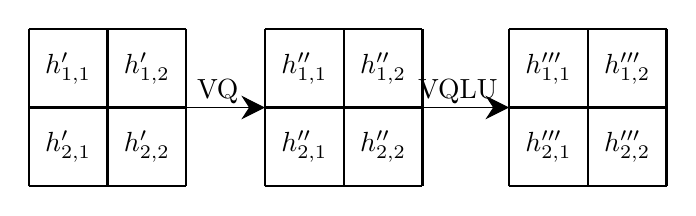
\begin{tikzpicture}
			\draw[thick, color=black] (0.0,0.0) grid (2, 2);
            
            \draw[thick, color=black, xshift=.0cm] (3,0.0) grid (5, 2);

            \draw[thick, color=black, xshift=.1cm] (6,0.0) grid (8, 2);
   
			%\draw[thick, step=1.0, color=blue, xshift=4.2cm] (0, 0) grid (1.0, 4);
			%\draw[thick, xstep=1.5, color=red, xshift=-2.0cm] (0, 0) grid (1.5, 4);

			%\node[draw=none, yshift=2cm, xshift=-.26cm] (eq) {$=$};
            \node [draw=none, yshift=1.5cm, xshift=0.5cm] () {$h'_{1,1}$};
            \node [draw=none, yshift=1.5cm, xshift=1.5cm] () {$h'_{1,2}$};
            \node [draw=none, yshift=0.5cm, xshift=0.5cm] () {$h'_{2,1}$};
            \node [draw=none, yshift=0.5cm, xshift=1.5cm] () {$h'_{2,2}$};

            \node [draw=none, yshift=1.5cm, xshift=3.5cm] () {$h''_{1,1}$};
            \node [draw=none, yshift=1.5cm, xshift=4.5cm] () {$h''_{1,2}$};
            \node [draw=none, yshift=0.5cm, xshift=3.5cm] () {$h''_{2,1}$};
            \node [draw=none, yshift=0.5cm, xshift=4.5cm] () {$h''_{2,2}$};

            \node [draw=none, yshift=1.5cm, xshift=6.6cm] () {$h'''_{1,1}$};
            \node [draw=none, yshift=1.5cm, xshift=7.6cm] () {$h'''_{1,2}$};
            \node [draw=none, yshift=0.5cm, xshift=6.6cm] () {$h'''_{2,1}$};
            \node [draw=none, yshift=0.5cm, xshift=7.6cm] () {$h'''_{2,2}$};

           \draw[-{Stealth[length=0.3cm, width=0.3cm]}] (2,1) -- node [yshift=.2cm, xshift=-.1cm]{VQ} (3,1); 
           \draw[-{Stealth[length=0.3cm, width=0.3cm]}] (5,1) -- node [yshift=.2cm, xshift=-.1cm]{VQLU} (6.1,1); 
			%\node<2> [draw=none, yshift=3.5cm, xshift=.5cm] (eq) {$a_{0,0}$};
			%\node<2> [draw=none, yshift=3.5cm, xshift=1.5cm] (eq) {$a_{0, 1}$};
			%\node<2> [draw=none, yshift=3.5cm, xshift=2.5cm] (eq) {$a_{0, 2}$};
			%\node<2> [draw=none, yshift=3.5cm, xshift=3.5cm] (eq) {$a_{0, 3}$};
            %\draw[thick, color=black, xshift=.2cm] (3,0.0) grid (5, 2);
			
		\end{tikzpicture}
        \caption{The vector quantization process on the latent space (in this example, the latent space is of size $2\times 2$). The output of the adapter layer, $h'_{i,j}$, is first quantized using VQ, resulting in the discrete grid $h''_{i,j}$. Then, the values $h''_{i,j}$ are used to look up (VQLookUp) the dictionary items from $D^{\widehat c}$, resulting in a continuous grid with elements $h'''_{i,j} \in \mathbb R^\latentdim$.}
        \label{fig:grid}
    
\end{figure}


%also talk about partitioning here

To train the proposed posthoc interpretation model, we use the training objective defined in the original VQ-VAE paper \cite{vqvae_vanoord}, such that the training loss $\mathcal L$ is defined as,
\begin{align}
    \mathcal L = d(x_\text{out}\| x) + \| h' - \text{sg}(h''') \|_2^2 + \| \text{sg}(h') - h''' \|_2^2  
\end{align}

where $d(x_\text{out}\| x)$, denotes the reconstruction error, and $\text{sg}(.)$ denotes the stop gradient operation.

%where $x_\text{int} =\text{Decoder}(h''')$, $h'''=D^{\widehat c}_{h''}$

%\franz{maybe another subsection? def link to an experimental results section}
% Mirco's version
It is worth noting that this formulation offers two options for using $x_\text{out}$ to generate the final interpretation $x_\text{int}$. The choice depends on the type of data being used. For data that requires continuous output, such as the Fashion MNIST dataset, the interpretation is obtained such that $x_\text{int}=x_\text{out}$, and the reconstruction error is calculated using $l_2$ loss during training. For binary images, such as MNIST and Quickdraw images, or audio, the model is trained with binary targets (obtained by thresholding the spectra for audio). In this case, the output of the model has a sigmoid activation function and the reconstruction error is computed using negative Bernoulli log-likelihood. The interpretation is then obtained by element-wise multiplying the input with the model output, such that $x_\text{int} = x \odot x_\text{out}$. In both cases, the classifier input is not affected.

%Note that this formulation allows two ways of using $x_\text{out}$ to produce the final interpretation $x_\text{int}$. The choice is dependent upon the data domain. For data that requires continuous output (such as the Fashion MNIST dataset in out experiments) we set $x_\text{int} =x_\text{out}$, and use $l_2$ loss for the reconstruction error during training. For binary images (MNIST and Quickdraw images), or audio however, we train the model with binary targets (which can be obtained by simply thresholding the spectra for audio), use a negative Bernoulli log-likelihood as the reconstruction error, and have sigmoid activation function at the output of the model. The interpretation is then obtained by masking the input data by element-wise multiplying the input with the model output such that $x_\text{int} = x \odot x_\text{out}$. Note in both cases, the classifier input is not affected.  
%and the model is able to produce interpretations. 


%Another interesting aspect of our approach is that it is very versatile, as it can work either as a masking approach or as a generator. 

%In the masking formulation, the interpretation is derived using an element-wise multiplication between the classifier input and the decoder's output. (reference to Fig 2). We use this approach for experiments on MNIST, Quickdraw, and ESC50, as it is beneficial for binary images and use cases where segmenting or thresholding the input is an option, like for audio. Otherwise, the decoder's output is treated directly as the interpretation in the generator formulation, as per FashionMNIST. Both approaches are valid for posthoc interpretability.
%
%The masking approach guarantees perfect alignment between interpretation and input in the input domain. However, it requires an explicit definition of binary targets for the VQ reconstruction, which can be achieved via thresholding, a segmentation network, or user-defined concepts similar to \cite{}. On the other hand, the generative formulation does not mathematically guarantee perfect alignment (although we experimentally validate the approach in Sec \ref{sec:quanteval}) but is more flexible and can handle any data domain and learning paradigm. This flexibility is a direct consequence of the interpreter network design and training strategy, which resembles the well-validated VQ-VAE model.
%%The training loss consists of ... 

% maybe a picture to show what's happening in the latent space with partitioning -- done, fig3

%\subsection{The training loss}
%talk about the loss func here

\section{Experiments} 

\subsection{Datasets and Model Details for Images}
\label{sec:datasetsandmodelingimages}

%In order to quantitatively and qualitatively on multiple domains, i.e. computer vision and audio analytics, 

% Mirco's version (minor changes)

We evaluated PIQ both qualitatively and quantitatively on three image datasets: MNIST \cite{lecun-mnisthandwrittendigit-2010}, FashionMNIST \cite{xiao2017fashionmnist}, and Quickdraw \cite{quickdraw}.For the Quickdraw dataset, we used a subset containing the ten classes used to evaluate FLINT \cite{FLINT}.

We employed the same classifier architecture for all three datasets. Specifically, we used a convolutional neural network with two convolutional blocks followed by max-pooling and a linear classifier at the end. The classification performance on MNIST, FashionMNIST, and Quickdraw datasets were $99.5\%$, $92.5\%$, and $87.0\%$, respectively. For more information on the classifier and architecture, please refer to Appendix \ref{app:design}.
%We evaluate PIQ qualitatively and quantitatively on three image datasets. We used MNIST \cite{lecun-mnisthandwrittendigit-2010}, FashionMNIST \cite{xiao2017fashionmnist}, and Quickdraw \cite{quickdraw} datasets. For Quickdraw, we used a subset containing the same 10 classes used to evaluate FLINT \cite{FLINT}. 
%We used the same classifier architecture for MNIST, Quickdraw, and FashionMNIST. Specifically, for all datasets, we used a convolutional neural network with two convolutional blocks followed by max-pooling and a linear classifier at the end. The classification performances that we obtained on MNIST, FashionMNIST and Quickdraw datasets are respectively $99.5\%$, $92.5\%$, and $87.0\%$. Details on the classifier and architecture can be found in Appendix \ref{app:design}.
%showcased in Table \ref{table:quantimages}. 
As input for the interpreter, we took the output of the second convolutional block of the classifier, a 4x4x128 tensor. The interpreter decoder consists of transposed convolutional layers (as described in Appendix \ref{app:design}). For all experiments, we used a codebook of 128-dimensional vectors with a total number of 256 vectors. We uniformly divided the dictionary over classes. For Quickdraw and MNIST datasets, the model output is used to mask the input such that $x_\text{int} = x \odot x_\text{out}$. For FashionMNIST the model output is used as an interpretation directly such that $x_\text{int} = x_\text{out}$, as described in Section \ref{sec:vq}.

%For we use the ESC50 dataset \cite{Piczak2015ESCDF}. 
% Mirco's verion
For the baselines, we used the original implementations of \href{https://github.com/jayneelparekh/flint}{FLINT} and \href{  https://github.com/marcotcr/lime}{LIME}, which can be found on the respective GitHub repositories. For VIBI, we used a \href{https://github.com/willisk/VIBI}{recent GitHub repository}. For L2I, we used our own implementation and adapted the method to work on images as well. Additional information on the L2I implementation for images can be found in the Appendix \ref{sec:l2iimpl}. The implementation of PIQ can be found in Speechbrain\footnote{\url{https://github.com/speechbrain/speechbrain/tree/develop/recipes/ESC50}}. 

%Our code is included as a supplemental meterial to this submission.

%For the baselines, we used the original implementations of \href{https://github.com/jayneelparekh/flint}{FLINT}, and \href{https://github.com/marcotcr/lime}{LIME}. For VIBI, we used a \href{https://github.com/willisk/VIBI}{recent repository}, and for L2I, we used our own implementation, and adapted the method to work on images as well. Details on the L2I implementation for images are explained in Appendix \ref{sec:l2iimpl}. Our code is attached to the submission.

%\cem{We need to talk about how we implemented the other methods, and say that we have used the same classifier for all.} %  Also talk about any data normalization. } 
%\newpage
\subsection{Quantitative Evaluation on Images}
\label{sec:quanteval}

% \textbf{92.9 $\pm$ 0.4} & \textbf{0.740 $\pm$ 0.021} & \textbf{0.018 $\pm$0.0001}
\begin{table*}[t]
\caption{Quantitative evaluation of interpretation quality on image datasets}
\label{table:quantimages}
\vskip 0.15in
\begin{center}
%\begin{small}
%\begin{sc}


\resizebox{13.9cm}{!}{
\begin{tabular}{l|ccc|ccc}
\toprule
 \textbf{Dataset}  & \multicolumn{3}{c|}{MNIST} & \multicolumn{3}{c}{FMNIST}  \\
 \midrule
\textbf{Metric} & Fidelity-In ($\uparrow$) & Faithfulness ($\uparrow$) & FID ($\downarrow$) & Fidelity-In ($\uparrow$) & Faithfulness ($\uparrow$) & FID ($\downarrow$) \\
\midrule
 PIQ (ours) & \textbf{98.03 $\pm$ 0.05} & \textbf{0.588 $\pm$ 0.00021} & \textbf{0.029 $\pm$ 0.0004}  & 
 \textbf{81.3 $\pm$ 0.2} & \textbf{0.773 $\pm$ 0.004} &  \textbf{0.030 $\pm$ 0.0004} \\ 


 VIBI & 73.90 $\pm$ 16.08 & 0.369 $\pm$ 0.002 & 0.710 $\pm$ 0.962 & 42.4 $\pm$ 17.8 & 0.578 $\pm$ 0.073 & 0.395 $\pm$ 0.104 \\
 
 L2I & 96.56  $\pm$ 2.66 & 0.453 $\pm$ 0.002 & 0.160 $\pm$ 0.010 & 68.3 $\pm$ 1.5
 & 0.343 $\pm$ 0.011 & 0.188 $\pm$ 0.011
 \\
 FLINT & 10.9 & 0.361 & 0.677 & 15.37 & -0.097 & 0.482 \\
\bottomrule
\end{tabular}
}
\newline

\resizebox{10.1cm}{!}{
\begin{tabular}{l|ccc}
\toprule

 \textbf{Dataset} & \multicolumn{3}{c}{Quickdraw}\\
 \midrule
\textbf{Metric} & Fidelity-In ($\uparrow$) & Faithfulness ($\uparrow$) & FID ($\downarrow$)\\
\midrule
 PIQ (ours) & \textbf{60.89 $\pm$ 0.60}& \textbf{0.675 $\pm$ 0.005} & \textbf{0.034 $\pm$ 0.0001}\\
 VIBI & 26.36 $\pm$ 3.01& 0.341 $\pm$ 0.031 &  0.388 $\pm$ 0.032\\
 L2I & 25.97 $\pm$ 0.82& 0.340 $\pm$ 0.031& 0.397 $\pm$ 0.020\\
 FLINT & 15.62 & -0.057 & 0.672 \\
\bottomrule 
\end{tabular}
}

%\end{sc}
%\end{small}
\end{center}
\vskip -0.1in
\end{table*}

\textbf{Metrics} 

% Mirco's version
To evaluate the quality of the generated interpretations quantitatively, we use three metrics. The first one is the fidelity-to-input, which is proposed in this paper for the first time. The second metric, Fréchet-Inception-Distance (FID) \cite{heusel2017gans}, that was previously used to asses the quality of the interpretations. Lastly, we use faithfulness \cite{alvarez2018} as our third metric.

%We use three metrics to compare the quantitative quality of the produced interpretations. The first is fidelity-to-input that we propose in this paper. Second, we propose to use Fréchet-Inception-Distance (FID) \cite{heusel2017gans} to measure the quality of the interpretations, and finally we use faithfulness \cite{alvarez2018}. 

% Mirco's verions
We define the metric of fidelity-to-input as the percentage agreement between the classifier's predictions for the original input and the interpretation. Mathematically, we express the fidelity-to-input (FID-I) as: \begin{align}
    \text{FID-I} = \frac{1}{N} \sum_{n=1}^N \left [\arg \max_c f_c(x_n) = \arg \max_c f_c(x_{\text{int}, n}) \right ], 
\end{align}
where $f_c(.)$ is the classifier's output probability for class $c$, and $[.]$ is the Iverson bracket which is 1 if the statement is true, and 0 if it is false. $x_n$ is the $n$'th data item, and $x_{\text{int}, n}$ is the interpretation that corresponds to the same input. This metric aims to measure how aligned the generated interpretations are to the original input in terms of the class predicted by the classifier. Ideally, the produced interpretation should not deviate from the original classifier decision. For example, the interpretation of a handwritten digit should not be classified as another digit.

%We define fidelity-to-input as the agreement, in percentage, between the predictions of the classifier for the original input and for the interpretation. Mathematically, we define the fidelity-to-input (FID-I) metric as follows, 
%\begin{align}
%    \text{FID-I} = \frac{1}{N} \sum_{n=1}^N \left [\arg \max_c f_c(x_n) = \arg \max_c f_c(x_{\text{int}, n}) \right ], 
%\end{align}
%where $f_c(.)$ denotes the classifier output probability for class $c$, and $[.]$ is the Iverson bracket where if the argument is true, the value of the bracket is 1, otherwise it is 0, $x_n$ is the $n$'th data item, and $x_{\text{int}, n}$ is the interpretation that corresponds to the same input. This metric aims to measure how aligned the generated interpretations are with respect to the original input in terms of class predicted by the classifier. Ideally, the produced interpretation should not deviate from the original classifier decision. For example, the interpretation of a handwritten digit should not be classified as another digit. 

%In the case of audio, the interpretation of a particular sound event should not be classified as a different sound event. -- removing this for now

As we mentioned in the introduction, with PIQ, we aim to generate interpretations that humans understand. Therefore, we want interpretations that are easy to associate with the original data distribution in the input space (pixel space for images). For this reason, we propose to use the Frechet-Inception Distance (FID) \cite{heusel2017gans} between the produced interpretations and the input data as an additional metric to describe the quality of interpretations. FID is a commonly used distance to measure the deviation between the distribution of the data generated by a generative model and the original data distribution. In this work, we use the original FID definition, and we extract image embeddings using an Inceptionv3 \cite{Szegedy2014GoingDW} network trained on ImageNet \cite{Russakovsky2014ImageNetLS} and compute the Fréchet Distance on the two Gaussian distributions estimated using the embeddings.

%\franz{Added details here, please check. Do you think we should have a formula too?}
% cem: looks pretty good to me! there is one reference I will add here also need to find it

Finally, we also measure the faithfulness of the interpretations. The faithfulness metric aims to measure the importance of the interpretation to the classifier decision. By following the way L2I \cite{parekh2022listen} defines this metric, we calculate the faithfulness as,
\begin{align}
    \text{Faithfulness} = f_{\widehat c} (x) - f_{\widehat c}(x - x_\text{int}), \label{eq:faithfulness}
\end{align}
where $f_{\hat{c}}(x)$ denotes output probability for the class that corresponds to the classifier decision $\widehat c$. For example, on the overlapping digit example showcased in the introduction, if the interpretation $x_\text{int}$ recovers the original digit perfectly, subtracting it from the input data $x$ would result in a low probability in the second term of the faithfulness definition given in equation \eqref{eq:faithfulness}.  

\textbf{Quantitative Performance Evaluation}

In Table \ref{table:quantimages}, we compare the quantitative metrics defined above on the three datasets mentioned in Section \ref{sec:datasetsandmodelingimages}. We compare PIQ with several prominent posthoc interpretation algorithms, which include FLINT \cite{FLINT}, VIBI \cite{VIBI}, and Listen-to-Interpret (L2I) \cite{parekh2022listen}. 


We train and evaluate all the methods on clean data from their respective train and test sets. To account for training variability, we perform three runs for all methods except for FLINT, as we found its performance to be consistently worse than other methods).  

%for which the AM+PI procedure to generate the hard to parallelize and therefore took a lot to compute for the entire test set. Another reason we considered when choosing to avoid running three separate runs for FLINT is the low performance on the single run, combined with the low qualitative performance observed in the user study that makes this approach less relevant for the comparison with PIQ.
%\cem{We need to comment on the fact that we did 3 runs, and 1 run for flint, need to talk about implementation details of L2I on images}

% Mirco's version
We found that PIQ outperforms the other methods in terms of FID-I, faithfulness, and FID. Furthermore, our results indicate that PIQ generates interpretations that are more closely aligned with the original data distribution, as evidenced by its lower Frechet Inception Distance (FID) values and higher fidelity-to-input (FID-I) scores. Overall, PIQ demonstrates superior performance in generating human-understandable interpretations.
%We observe that PIQ results in superior performance in terms of FID-I, faithfulness, and FID. Moreover, we conclude that PIQ stays closer to the original data distribution than the other methods, as showcased by lower Frechet Inception Distance (FID) and larger fidelity-to-input (FID-I) values. 

%\cem{We might want to comment further on this once we get all the numbers}. 

%\franz{These results are all on clear samples} 





\subsection{Qualitative Evaluation on Images}
\label{sec:images-qualitative} 
\textbf{Experiment description} 

\begin{figure*}[h!]
    \centering
    \includegraphics[width=0.16\textwidth]{mnistmixtures/samples.png}
    \includegraphics[width=0.16\textwidth]{mnistmixtures/superpose_ours.png}
    \includegraphics[width=0.16\textwidth]{mnistmixtures/superpose_VIBI.png}
    \includegraphics[width=0.16\textwidth]{mnistmixtures/superpose_L2I.png}
    \includegraphics[width=0.16\textwidth]{mnistmixtures/superpose_lime.png}
    \includegraphics[width=0.16\textwidth]{mnistmixtures/superpose_FLINT.png}

    \includegraphics[width=0.16\textwidth]{fmnistmixtures/samples.png}
    \includegraphics[width=0.16\textwidth]{fmnistmixtures/superpose_masks.png}
    \includegraphics[width=0.16\textwidth]{fmnistmixtures/superpose_VIBI.png}
    \includegraphics[width=0.16\textwidth]{fmnistmixtures/superpose_L2I.png}
    \includegraphics[width=0.16\textwidth]{fmnistmixtures/superpose_lime.png}
    \includegraphics[width=0.16\textwidth]{fmnistmixtures/superpose_FLINT_interpretations.png}

    \includegraphics[width=0.16\textwidth]{fmnistonmnist/samples.png}
    \includegraphics[width=0.16\textwidth]{fmnistonmnist/superpose_ours.png}
    \includegraphics[width=0.16\textwidth]{fmnistonmnist/superpose_VIBI.png}
    \includegraphics[width=0.16\textwidth]{fmnistonmnist/superpose_L2I.png}
    \includegraphics[width=0.16\textwidth]{fmnistonmnist/superpose_lime.png}
    \includegraphics[width=0.16\textwidth]{fmnistonmnist/superpose_FLINT_interpretations.png}
    
    \includegraphics[width=0.16\textwidth]{quickdraw0db/samples.png}
    \includegraphics[width=0.16\textwidth]{quickdraw0db/superpose_ours.png}
    \includegraphics[width=0.16\textwidth]{quickdraw0db/superpose_VIBI.png}
    \includegraphics[width=0.16\textwidth]{quickdraw0db/superpose_L2I.png}
    \includegraphics[width=0.16\textwidth]{quickdraw0db/superpose_lime.png}
    \includegraphics[width=0.16\textwidth]{quickdraw0db/superpose_FLINT_overlap.png}

    \includegraphics[width=0.16\textwidth]{quickdraw37/samples.png}
    \includegraphics[width=0.16\textwidth]{quickdraw37/superpose_ours.png}
    \includegraphics[width=0.16\textwidth]{quickdraw37/superpose_VIBI.png}
    \includegraphics[width=0.16\textwidth]{quickdraw37/superpose_L2I.png}
    \includegraphics[width=0.16\textwidth]{quickdraw37/superpose_lime.png}
    \includegraphics[width=0.16\textwidth]{quickdraw37/superpose_FLINT_overlap.png}
    
    
    \caption{Comparing interpretation methods on overlapped data. The interpretations are highlighted in red overlays. The top row shows overlapping MNIST digits, with classifier decisions indicated on the top right corner of each digit. The second row shows overlapping FashionMNIST data items, the third row shows MNIST digits with FashionMNIST backgrounds, and the fourth and fifth rows show overlapping Quickdraw drawings with different weights. The leftmost image shows the overlapping input given to the classifier, with the following images showing interpretations generated by PIQ, VIBI, L2I, LIME, and FLINT respectively.}
    \label{fig:overlapmnist}
\end{figure*}

% Mirco's version
To evaluate the effectiveness of our method in handling challenging data, we performed tests on contaminated inputs. We compared various methods for generating contaminated data, specifically:

\begin{itemize}
    \item \textbf{(Case1)} Overlapping Handwritten digits from the MNIST dataset \cite{lecun-mnisthandwrittendigit-2010}
    \item \textbf{(Case2)} Overlapping Clothing items from the FashionMNIST dataset \cite{xiao2017fashionmnist} 
    \item \textbf{(Case3)} Handwritten digits with background with samples from the FashionMNIST dataset.
    \item \textbf{(Case4)} Overlapping Handdrawings from the Quickdraw dataset \cite{quickdraw} We have two versions where i) We overlap the images with equal weights (v1) ii) We overlap the images with weights 0.7 and 0.3 (v2).
\end{itemize}

%To qualitatively assess our method on challenging data, we have tested our method on data with contamination. Namely, we compared several different methods on data contaminated with other samples. More precisely, here is the list of conditions under which we evaluate the interpretation methods: 
%\begin{itemize}
%    \item \textbf{(Case1)} Overlapping Handwritten digits from the MNIST dataset \cite{lecun-mnisthandwrittendigit-2010}
%    \item \textbf{(Case2)} Overlapping Clothing items from the FashionMNIST dataset \cite{xiao2017fashionmnist} 
%    \item \textbf{(Case3)} Handwritten digits with background with samples from the FashionMNIST dataset.
%    \item \textbf{(Case4)} Overlapping Handdrawings from the Quickdraw dataset \cite{quickdraw} We have two versions where i) We overlap the images with equal weights (v1) ii) We overlap the images with weights 0.7 and 0.3 (v2).
%\end{itemize}

In Figure \ref{fig:overlapmnist}, we present the interpretations generated by PIQ, VIBI, L2I, LIME, and FLINT on the challenging data setups outlined above. It's worth mentioning that the classifier predictions for cases 2, 4-i, and 4-ii can be found in Appendix \ref{sec:extrapiqsamples}. 

%We observe that the most intuitive interpretations are the ones generated with PIQ. 

% Mirco's version
As the low FID values in Table \ref{table:quantimages} suggest, PIQ preserves the distribution of the handwritten digits much better than the other algorithms. While VIBI sometimes generates interpretations that resemble digits, they often deviate from the classifier's decision, as indicated by the green indicators on the top right corner. L2I generally produces better interpretations than VIBI, but still does not attain the level of distribution preservation achieved by PIQ. LIME simply reproduces the input mixture without altering it, while FLINT's generated interpretations, even though they may contain the original digits, do not meet the criterion of understandability.

%For the overlapping MNIST digits (case 1), as hinted by the low FID obtained by PIQ on clean digits on Table \ref{table:quantimages}, the interpretations obtained with PIQ preserve the distribution of the handwritten digits much better than the other algorithms. Although VIBI obtains some interpretations that resemble digits, it often results in an interpretation that does not correspond to the classifier decision shown in the top right corner with green indicators. L2I in general obtains better interpretations than VIBI, but still does not attain the level of distribution-match obtained by PIQ. We observe that LIME does not alter the input mixtures, and results in returning the overlapping digit image as is. For FLINT, we consider the most relevant attribute generated using the local interpretation algorithm described in the original paper and the original PyTorch implementation. However, we observe that even though the images sometimes contain the original digits, the resulting interpretations do not generally satisfy the understandability criterion.

We observe a similar behavior on the overlapping FashionMNIST items (second row of Figure \ref{fig:overlapmnist}), and MNIST digits with Fashion MNIST background (third row of Figure \ref{fig:overlapmnist}) as well. PIQ obtains explanations that remain aligned with the classifier decision, the interpretations are easy to understand, and remain loyal to the original data distribution. Finally, on overlapping Quickdraw drawings (shown in the fourth row for the equal weight mixing case, and the fifth row for the case with weights 0.7 and 0.3 in Figure \ref{fig:overlapmnist}), we see that especially on the equal weight mixing case, the methods mostly fail to produce meaningful explanations as the mixtures are challenging. LIME can generate some explanations that are understandable, but do not provide any substantial intuition that is not already found in the input image. We however observe that PIQ produces explanations that generally correlate well with the classification decisions of the classifier. Note that we provide the list of classifier decisions in $4\times4$ grid format in Appendix \ref{sec:extrapiqsamples}.   

%\cem{We can now talk about some qualitative experiments on FMNIST, and Quickdraw}. 

\textbf{User Study} \\
To measure human preference towards the different interpretation methods, we performed a user study, in which we compared several different interpretation methods. 

%We aim to identify the user preferences for the interpretations obtained from challenging data, i.e. overlapping samples for MNIST, FashionMNIST, and Quickdraw with a cluttered background.

For each overlapping data case described above, we asked the participants to rate the quality of the interpretations with a score between 1 (bad) and 5 (excellent). For each case, we showed each participant 16 different images presented in a $4\times 4$ format (similar to the images in Figure \ref{fig:overlapmnist} - For case-1 we studied two batches). We first showed the participants the overlapping inputs that were given to the classifier, and then we followed up with the interpretations obtained with PIQ, VIBI, FLINT, L2I, and LIME (presented in random order). For the studies corresponding to cases 1,2,3,4 we had 23, 16, 22, and 20 participants respectively. 

%For case 1 (overlapping MNIST digits) we showed the participants two batches of 16

% Mirco's version
Table \ref{table:mosimages} displays the mean opinion scores for different interpretations using various approaches in all 4 cases. We can see that the interpretations produced by PIQ are consistently preferred by participants. In the overlapping MNIST case (case-1), there was no close contender. In case-2 (Fashion-MNIST mixtures), L2I was the second-best method in terms of participant preference. However, it's worth noting that PIQ received a score of 5 (excellent) from 15 participants, while only receiving 3 from one participant. In cases 3 and 4, LIME was the closest contender, as their interpretations tend to closely resemble the input image. However, LIME was less preferred in balanced mixtures of case 1 and 2, and more preferred in imbalanced mixtures of case 3 and 4-ii. It's also worth noting that for case 4-i and 4-ii, the study was limited to PIQ and LIME as these two methods seemed to produce the best results as seen in Figure \ref{fig:overlapmnist}.

%In Table \ref{table:mosimages}, we show the mean opinion scores for the different approaches on different interpretations for all 4 cases. We observe in all cases that the interpretations obtained by PIQ are preferred by the participants. In the overlapping MNIST case (case-1), we have not observed a close contender. In case-2, (Fashion-MNIST mixtures) L2I was the second best method in terms of the participant preference. However, we would like to indicate that PIQ obtained a score of 5 (excellent) from 15 participants and 3 from just one participant. We have observed that for case-3 and case-4 the closest contender was LIME, as in general LIME interpretations tend to return interpretations that  almost identically resemble the input image. In case-3 and especially case-4-ii since the mixtures are imbalanced (one of the classes is more present than the other) a conservative approach such as LIME generally tends to be preferred by participants, but we observe that LIME is less preferred in the balanced mixtures of case1 and case2. Also note that, for cases 4-i and 4-ii, we have limited the study to PIQ and LIME, as these two seemed to produce the two best qualitative results as can be seen from Figure \ref{fig:overlapmnist}. 


% For case 1 (overlapping MNIST), we presented two batches of sixteen overlapping 

%We have presented the obtained interpretations with all of the methods and asked the users the following question: \emph{Which of these interpretations, in your opinion, best describes the predicted class for these mixtures?}. For overlapping MNIST digits, we have shown five batches of 16 images to 20 users. \franz{maybe this last thing might go in Appendix?}
%\cem{We can do a }


\begin{table}[t]
\caption{Sujective evaluation of interpretation quality on overlapping images}
\label{table:mosimages}
\vskip 0.15in
\begin{center}
\begin{small}
\begin{sc}
\resizebox{7.1cm}{!}{
\begin{tabular}{l|c|c}
\toprule
Dataset & Method & MOS ($\uparrow$)\\
\midrule
   \multirow{5}{*}{MNIST B1}& PIQ (ours) & \textbf{4.04 $\pm$ 0.48}   \\
  & VIBI &  1.77 $\pm$ 0.68 \\
 \multirow{3}{*}{(Case 1)}& L2I &  2.4 $\pm$ 0.66 \\
 & FLINT & 1 $\pm$ 0    \\
 & LIME  & 2 $\pm$ 1.34 \\
 \midrule
  \multirow{5}{*}{MNIST B2}& PIQ (ours) & \textbf{3.95 $\pm$ 0.72}   \\
 & VIBI &  1.86 $\pm$ 0.71  \\
 \multirow{3}{*}{(Case 1)}& L2I &  1.86 $\pm$ 0.56 \\
 & FLINT &  1.04 $\pm$ 0.21    \\
 & LIME &  2.13 $\pm$ 1.21 \\
 \midrule

% \multirow{5}{*}{FMNIST Mix} & PIQ (ours) & \textbf{3.95 $\pm$ 0.78}   \\
% & VIBI &  1 $\pm$ 0  \\
% \multirow{3}{*}{(Case 2)}& L2I &   2.77$\pm$ 0.75 \\
% & FLINT &  1.09 $\pm$ 0.29    \\
% & LIME &  2.40 $\pm$ 0.96 \\
 
 \multirow{5}{*}{FMNIST Mix} & PIQ (ours) & \textbf{4.87 $\pm$ 0.50}   \\
 & VIBI &  1.37 $\pm$ 0.50 \\ 
 \multirow{3}{*}{(Case 2)}& L2I & 3.18$\pm$ 0.91 \\
 & FLINT &  1.12$\pm$ 0.50    \\
 & LIME &  1.37 $\pm$ 0.89 \\
  \midrule
 \multirow{5}{*}{MNIST+FMN} & PIQ (ours) & \textbf{4.78 $\pm$ 0.43}   \\
 & VIBI &  1.14 $\pm$ 0.47  \\
 \multirow{3}{*}{(Case 3)}& L2I &  2.18 $\pm$ 0.96 \\
 & FLINT &  1.09 $\pm$ 0.47    \\
 & LIME &  3.23 $\pm$ 0.72 \\
   \midrule
 \multirow{1}{*}{QuickDraw1} & PIQ (ours) & \textbf{2.6 $\pm$ 1.67}   \\
 (Case4-i)& LIME &  {2.35 $\pm$ 1.46}  \\
   \midrule
 \multirow{1}{*}{QuickDraw2} & PIQ (ours) & \textbf{3.55 $\pm$ 1.0}   \\
(Case4-ii) & LIME &  3 $\pm$ 1,38 \\
\bottomrule
\end{tabular}
}
\end{sc}
\end{small}
\end{center}
\vskip -0.1in
\end{table}



\subsection{Qualitative Interpretation Study on Audio}
\textbf{Dataset and Modeling Details} \\
We test the interpretations produced by PIQ on the ESC-50 dataset \cite{Piczak2015ESCDF}, which consists of 2000, 5 seconds-long clips of 50 different classes of sound events. Example sound events in the dataset include 'cat', 'dog', 'baby cry', 'church-bells', and so on.  

% Mirco's version
As a classifier, we utilized a convolutional network consisting of four strided 2D-convolutional layers with a downsampling factor of 2. Each layer is followed by batch normalization and ReLU activation. The network ends with a residual convolutional layer before a linear classifier. We pretrained the convolutional layers on the VGGSound dataset \cite{Chen20}, which comprises around 550 hours of audio clips sourced from Youtube. The classifier operates in the log-spectrogram domain and achieved 75\% classification accuracy on fold-4 of the ESC50 dataset when trained on folds 1-2-3. We worked with 16kHz audio, using a 1024 point FFT, with a 23ms window-length and 11ms hop length. To balance the distribution of frequencies, we applied a log-transform to the magnitude spectrogram.

%As a classifier, we used a convolutional classifier that consists of four strided 2D-convolutional layers with a downsampling factor of 2. Each layer is followed by batch-norm and ReLU non-linearity, and a residual convolutional layer at the end before a linear layer for classification. We pretrained the convolutional layers on the VGGSound dataset \cite{Chen20} which consists of around 550 hours of audio clips that are collected from Youtube. The classifier works on the log-spectrogram domain and achieves a performance of 75\% classification accuracy on the fold-4 of the ESC50 dataset when trained on folds 1-2-3. We work with 16kHz audio, and use 1024 point FFT, with 23ms window-length and 11ms hop length. We apply a log-transform to the magnitude spectrogram to have more even distribution over the frequencies. 

% Mirco's version
 The output of the last layer of the classifier serves as input for the interpreter model. For the adapter, we employed a combination of a residual convolutional layer and a strided 2D convolutional layer. Detailed information on the neural network architectures can be found in Appendix \ref{app:design_audio}. The decoder comprises five layers of strided transposed-2D convolutions. The interpreter is trained on a clean dataset, specifically using folds 1-2-3 of the ESC50 dataset, which is the same dataset used for the classifier. To find a mask on the magnitude STFT, we use PIQ in binary-masking mode and apply a sigmoid nonlinearity at the encoder's output. To obtain the training data for PIQ, we set a threshold of $0.35*\max(X)$ for each spectrogram $X$. We utilized a total of 1024 dictionary items that are evenly distributed across the classes.
 
%We use the output of the last layer of the classifier before the linear output layer as input to the interpreter model. For the adapter, we use a residual convolutional layer combined with one strided 2D convolutional layer. We described the neural net architectures used in Appendix \ref{app:design_audio}. The decoder consists of 5 layers of strided transposed-2D Convolutional layers. As usual, we train the interpreter on the clean dataset, on folds 1-2-3 of the ESC50 dataset (same as the classifier). We use PIQ in the binary-masking mode, as the goal of the interpreter is to find a mask on the magnitude STFT, and therefore we use a sigmoid nonlinearity at the output of the encoder.  We used a threshold of $0.35*\max(X)$ for each spectrogram $X$ to get the training data for PIQ. We used 1024 dictionary items in total, with a uniformly divided dictionary over classes.  

\textbf{Qualitative Evaluation and User Study} 
\begin{figure*}[t]
    \centering
    \includegraphics[width=0.49\textwidth, trim=2cm 0.5cm 1cm 0cm,clip]{Set1_mos.pdf}
    \includegraphics[width=0.49\textwidth, trim=2cm 0.5cm 1cm 0cm,clip]{Set2_mos.pdf}
    \caption{Distribution of user opinion scores on the audio interpretations. Yellow circles indicate the average scores. (left) The distribution of the first set of audio recordings (taken from the official companion website of L2I). (right) Results obtained on audio mixtures we have created. In both sets, we color-coded the audio mixtures: the first recording is red, the second is blue, the third is green, and the fourth is black. The algorithms compared are PIQ (ours), L2I-1 (these are the official results of L2I that we downloaded from the L2I companion website), L2I-2 (these are the results we obtained with our L2I implementation).  }
    \label{fig:audio1}
\end{figure*}

% Mirco's version
As we did in Section \ref{sec:images-qualitative} for overlapping images, we examine the interpretation quality of classifier decisions on audio mixtures as well. It is worth recalling that the system is trained on clean signals, not on mixtures. The models we implemented work in the log-magnitude STFT domain, and we reconstruct the time-domain signal by inverting the filtered input magnitude spectrogram using the  phase of rhe input signal, a common practice in magnitude spectrogram-based source separation, as seen in \cite{deepclustering}.

%Similar to the overlapping image experiments in Section \ref{sec:images-qualitative}, we study the interpretation quality of classifier decisions on audio mixtures as well. We would like to again note that the system is trained on clean signals, and not on mixtures. The models that we implemented operate in the log-magnitude STFT domain, and the time-domain reconstruction is obtained by inverting the filtered input magnitude spectrogram using the phase of the input signal (as is commonly done in magnitude spectrogram based source separation, e.g. as in \cite{deepclustering}). 

% Mirco's verision
We compare our method with L2I, as it is recently shown to outperform alternatives for interpreting classifier decisions on audio data \cite{parekh2022listen}. To directly compare the qualitative difference between PIQ and L2I, we tested these methods on the four sound mixtures provided in the \href{https://jayneelparekh.github.io/listen2interpret/}{companion website of L2I}. In addition to these four mixtures, we also tested four different audio mixtures that we created from fold-4 of the ESC50 dataset.

%To directly compare the qualitative difference between L2I, a recent posthoc-interpretation method designed to interpret audio classifiers, we tested our method on the four sound mixtures provided in the \href{https://jayneelparekh.github.io/listen2interpret/}{companion website of L2I}. In addition to these four mixtures, we also tested 4 different audio mixtures that we created from the fold-4 of the ESC50 dataset.  

% Mirco's version
To rigorously study the user preference for the interpretations produced by PIQ and L2I, we conducted a user study with 22 participants. On the four sound mixtures provided in the companion website of L2I, we compared PIQ with two versions of interpretations from L2I. i) The results provided on the website (that is, the official results provided by the authors of L2I -- we denote this version with L2I-1) ii) Our implementation of L2I which uses the same classifier as PIQ, described above -- we denote this version with L2I-2. For the decoder network of L2I-2, we used a similar architecture that we used for PIQ, except that we had a pretrained NMF dictionary on the output of the convolutional decoder. We have shown the users the mixtures and then asked them to rate the interpretations provided PIQ, L2I-1, and L2I-2 between 1 (bad) and 5 (excellent). 

We show the result of this user study on the left panel of Figure \ref{fig:audio1}. We see that the participants consistently preferred PIQ over both versions of L2I. These audio interpretations along with the mixtures can be found on our companion website\footnote{\url{https://piqinter.github.io/}}.

%In order to rigorously study the user preference for the interpretations produced by PIQ and L2I, we conducted a user study with 22 participants. On the four sound mixtures provided in the companion website of L2I, we compared PIQ with two versions of interpretations from L2I. i) The results provided on the website (that is, the official results provided by the authors -- we denote this version with L2I-1) ii) Our implementation of L2I which uses the same classifier as PIQ, described above -- we denote this version with L2I-2. For the decoder network of L2I-2, we used a similar architecture that we used for PIQ, except that we had a pretrained NMF dictionary on the output of the convolutional decoder. We have shown the users the mixtures and then asked them to rate the interpretations provided PIQ, L2I-1, and L2I-2 between 1 (bad) and 5 (excellent). We show the result of this user study on the left panel of Figure \ref{fig:audio1}. We see that the participants consistently preferred PIQ over both versions of L2I. These audio interpretations along with the mixtures can be found on our companion website\footnote{\url{https://piqinter.github.io/}}. 

\begin{figure}[h!]
    \centering
    \includegraphics[width=.48\textwidth, trim=0cm 0.3cm 0cm 0cm,clip]{specs_new.png}
    %\vspace{-.3cm}
    \caption{Demonstration of PIQ on audio. (top-left) The dominant audio source, (top-right) Contaminating class, (bottom-left) Mixture, (bottom-right) Produced interpretation.}
    \label{fig:specs}
\end{figure}

% Mirco's version
As previously mentioned, we also compare the interpretation quality of PIQ on four additional mixtures that we created. In this case, we only compared with our implementation of L2I (L2I-2) that interprets the same classifier as PIQ. From the right panel of Figure \ref{fig:audio1}, we can see that users again prefer PIQ over L2I, as shown by the higher average opinion score (represented by yellow circles on top of the box plots).

%As mentioned before, we also compare the interpretation quality of PIQ on four other mixtures that we have formed. In this case, we have only been able to compare with our implementation of L2I, which operates on the same classifier as PIQ (L2I-2 mentioned above). We see from the right panel of Figure \ref{fig:audio1} that users again prefer PIQ over L2I in terms of average opinion score (shown by yellow circles on top of the box plots). 

% Mirco's version
An example of PIQ interpretation on audio can be seen in Figure \ref{fig:specs}. The input signal is a mixture of cat-meowing as the main class and hand clapping as the contaminating class. As shown on the bottom-right spectrogram, the clapping sound is concentrated in the lower half of the spectrum. On the bottom-right panel, we can see that PIQ effectively removes the background clapping noise and focuses on the harmonic of the cat-meowing sound. This interpretation can be found as the 4th mixture in the second section of our companion website \href{https://piqinter.github.io/}.
It is worth noting that we also examined the case where the classifier makes an incorrect classification (mixture 3-section 2 on the companion website) and found that PIQ still produces a relevant interpretation that accurately reconstructs a sound clip resembling the classifier decision 'Pig'."

%As an example interpretation, in Figure \ref{fig:specs}, we show the interpretation obtained with PIQ. The input signal consists of cat-meowing as the main class and hand clapping as the contaminating class. We see on the bottom right spectrogram that the clapping sound populates the lower half of the spectrum. We observe on the bottom right panel that PIQ removes the background clapping noise and focus on the harmonic cat meowing sound in the interpretation signal. This interpretation can be found as the 4th mixture in the second section of our \href{https://piqinter.github.io/}{companion website}.

%We would like to also note that we have also explored the case where the classifier makes a wrong classification (mixture 3-section 2 on the companion website) and we observe that PIQ produces a relevant interpretation that accurately reconstructs a sound clip that resembles the classifier decision 'Pig'. 

\section{Conclusions}
% Mirco's version:
In this paper, we proposed PIQ, a post-hoc method for interpreting neural network classifiers. Through a series of user studies on image and audio data, we showed that the interpretations generated by PIQ are preferred by participants over several alternative methods in the literature. Furthermore, we demonstrated that PIQ outperforms these baselines on quantitative metrics, and closely matches the original data distribution.\\
%PIQ offers a general framework for learning interpretable reconstructions of classifier representations. It's worth noting, however, that 

\textbf{Limitations:}
%In principle, PIQ can be applied to other forms of data, such as video, and text, however 
This study is limited to the application of PIQ to image and audio data. Additionally, we have not yet used our method to explain classifiers on more complex data, such as longer audio signals, or large color images. 
%object detection in large images or sound event detection in long audio signals.

%We proposed PIQ, a posthoc method to interpret neural network classifiers. Through several user studies we have shown on contaminated image data and audio data that the interpretations given by PIQ are preferred by participants over several baselines in the literature. We have also shown that in terms of closeness to the original data distribution, PIQ outperforms several baseline methods in the literature. 
%PIQ offers a general framework to learn reconstructions of classifier representations. \\
%\textbf{Limitations:}
%Even though we have considered images and audio in this paper, in principle PIQ can also be applied to other modalities such as video, multi-modal data, and text. We have also not considered more complex tasks such as object detection in large images, sound event detection in long audio signals.

\bibliography{example_paper}
\bibliographystyle{unsrtnat}


%%%%%%%%%%%%%%%%%%%%%%%%%%%%%%%%%%%%%%%%%%%%%%%%%%%%%%%%%%%%%%%%%%%%%%%%%%%%%%%
%%%%%%%%%%%%%%%%%%%%%%%%%%%%%%%%%%%%%%%%%%%%%%%%%%%%%%%%%%%%%%%%%%%%%%%%%%%%%%%
% APPENDIX
%%%%%%%%%%%%%%%%%%%%%%%%%%%%%%%%%%%%%%%%%%%%%%%%%%%%%%%%%%%%%%%%%%%%%%%%%%%%%%%
%%%%%%%%%%%%%%%%%%%%%%%%%%%%%%%%%%%%%%%%%%%%%%%%%%%%%%%%%%%%%%%%%%%%%%%%%%%%%%%
\newpage
\appendix
\onecolumn

\section{Samples for qualitative evaluation of PIQ on images}
\label{sec:extrapiqsamples}

In Figure \ref{fig:overlapmnist}, the interpretations are superimposed on the input samples, Here, we also show the interpretations as grayscale format in Figure \ref{fig:overlapmnist_bit}.

\begin{figure*}[h!]
    \centering
    \includegraphics[width=0.16\textwidth]{mnistmixtures/samples.png}
    \includegraphics[width=0.16\textwidth]{mnistmixtures/ours.png}
    \includegraphics[width=0.16\textwidth]{mnistmixtures/VIBI.png}
    \includegraphics[width=0.16\textwidth]{mnistmixtures/L2I.png}
    \includegraphics[width=0.16\textwidth]{mnistmixtures/lime.png}
    \includegraphics[width=0.16\textwidth]{mnistmixtures/FLINT.png}

    \includegraphics[width=0.16\textwidth]{fmnistmixtures/samples.png}
    \includegraphics[width=0.16\textwidth]{fmnistmixtures/masks.png}
    \includegraphics[width=0.16\textwidth]{fmnistmixtures/VIBI.png}
    \includegraphics[width=0.16\textwidth]{fmnistmixtures/L2I.png}
    \includegraphics[width=0.16\textwidth]{fmnistmixtures/lime.png}
    \includegraphics[width=0.16\textwidth]{fmnistmixtures/FLINT_interpretations.png}

    \includegraphics[width=0.16\textwidth]{fmnistonmnist/samples.png}
    \includegraphics[width=0.16\textwidth]{fmnistonmnist/ours.png}
    \includegraphics[width=0.16\textwidth]{fmnistonmnist/VIBI.png}
    \includegraphics[width=0.16\textwidth]{fmnistonmnist/L2I.png}
    \includegraphics[width=0.16\textwidth]{fmnistonmnist/lime.png}
    \includegraphics[width=0.16\textwidth]{fmnistonmnist/FLINT_interpretations.png}
    
    \includegraphics[width=0.16\textwidth]{quickdraw0db/samples.png}
    \includegraphics[width=0.16\textwidth]{quickdraw0db/ours.png}
    \includegraphics[width=0.16\textwidth]{quickdraw0db/VIBI.png}
    \includegraphics[width=0.16\textwidth]{quickdraw0db/L2I.png}
    \includegraphics[width=0.16\textwidth]{quickdraw0db/lime.png}
    \includegraphics[width=0.16\textwidth]{quickdraw0db/FLINT_overlap.png}

    \includegraphics[width=0.16\textwidth]{quickdraw37/samples.png}
    \includegraphics[width=0.16\textwidth]{quickdraw37/ours.png}
    \includegraphics[width=0.16\textwidth]{quickdraw37/VIBI.png}
    \includegraphics[width=0.16\textwidth]{quickdraw37/L2I.png}
    \includegraphics[width=0.16\textwidth]{quickdraw37/lime.png}
    \includegraphics[width=0.16\textwidth]{quickdraw37/FLINT_overlap.png}

    \resizebox{13.7cm}{!}{
\begin{tabular}{|l|l|l|l|}
\hline
Pullover & Pullover & Trouser & Trouser \\ \hline
Shirt & Trouser & Coat & Shirt \\ \hline
Trouser & Pullover & Coat & Sneaker \\ \hline
Ankle Boot & Dress & Coat & Dress \\ \hline
\end{tabular}
\quad 
\begin{tabular}{|l|l|l|l|}
\hline
Cow & Grapes & Lion & Carrot \\ \hline
Lion & Grapes & Lion & Lion \\ \hline
Lion & Lion & Grapes & Cow \\ \hline
Frog & Grapes & Lion & Lion \\ \hline
\end{tabular}
\quad
\begin{tabular}{|l|l|l|l|}
\hline
Grapes & Ant & Carrot & Frog \\ \hline
Lion & Grapes & Cow & Lion \\ \hline
Dog & Banana & Dog & Lion \\ \hline
Frog & Cow & Cow & Lion \\ \hline
\end{tabular}


}

\caption{Comparing interpretation methods on overlapping MNIST digits -  The classifier decisions are indicated on the top right corner of each digit with green text. (top), overlapping FashionMNIST data items (second row), MNIST digits with FashionMNIST backgrounds (third row), overlapping Quickdraw drawings (with equal weights for both images), overlapping Quickdraw drawings (with weights 0.7 and 0.3). The overlapping images that are input to the classifier are shown on the leftmost image. From left-to-right, interpretation images shown correspond to columns 2) PIQ (ours), 3) VIBI, 4) L2I, 5) LIME, 6) FLINT. The table at the bottom of the picture are (from left to right) predicted classes for the second row (case 2 mixtures), predicted classes for the fourth row (case4-i mixtures), and predicted classes for the last row (case4-ii mixtures).}
    \label{fig:overlapmnist_bit}
\end{figure*}

\newpage

\section{L2I adaptation for images}
\label{sec:l2iimpl}

Although L2I \cite{parekh2022listen} was initially presented for audio, the same approach can be applied to images. In particular, Non-Negative Matrix Factorization (NMF) - the core of the L2I approach - has several applications on images \cite{Lee1999LearningTP, Hoyer2004NonnegativeMF}. For the experiments in this paper, we used an NMF dictionary, $W \in \mathbb{R}^{100\times W\times H}$, composed of 100 components of the exact resolution as the original input image ($W\times H$). We kept the architecture of the $\Theta$ network in the original implementation as in the original paper. Thus, it has a pooling layer applied to the spatial dimension, followed by a linear layer, whose weights are used to compute each component's relevance. 
%To ensure the correct implementation of the approach, we checked the components of the pipeline with reconstruction and overfitting tests. 
%\franz{not sure if we need this}. 
%Sample reconstructions , are depicted in Figure \ref{fig:NMFrec}. 
%
%\begin{figure}[h]
%    \centering
%    \includegraphics[width=.235\textwidth]{NMF_recon.png}
%    % \includegraphics[width=.235\textwidth]{mnistmixtures/superpose_ours.png}
%    \caption{Showcasing NMF reconstructions on random samples from the considered datasets. From top to bottom: FashionMNIST, Quickdraw, and MNIST.}
%    \label{fig:NMFrec}
%\end{figure}

\section{Neural network design for Images}
\label{app:design}
For reproducibility, together with the code submitted with this paper we present here, in pseduocode, the main neural networks used in training PIQ for our experiments with images.

The naming convention for the layers is the one from PyTorch\footnote{https://pytorch.org/docs/stable/index.html}. For convolutional layers, $k$ is the kernel size, $s$ is the stride, and $p$ the padding. The classifier architecture is as follows:
% \lstinputlisting[language=Python]{BitXorMatrix.m}
\begin{Code}
    \begin{lstlisting}
    def classifier_forward(x):
        x = Conv2d(1, 32, k=3, s=1)(x)
        x = ReLU(x)
        x = Conv2d(32, 64, k=3, s=1)(x)
        x = ReLU(x)
        x = MaxPool2d(2, 2)(x)
        x = Dropout2d(p=0.25)(x)
        x = Conv2d(64, 64, k=3, s=1)(x)
        x = ReLU(x)
        x = Conv2d(64, 128, k=3, s=1)(x)
        x = ReLU(x)
        h = MaxPool2d(2, 2)(x) # this is the input for the adapter
        x = Linear(2048, 128)(h)
        x = ReLU(x)
        x = Dropout2d(p=0.5)(x)
        out = Linear(128, num_classes)(x)
        
        return x, h
    \end{lstlisting}
\end{Code}
The PIQ decoder forward pass is as follows:
\begin{Code}
    \begin{lstlisting}
    def decoder_forward(x):
        x = ResBlock(128)(x)
        x = ResBlock(128)(x)
        x = ReLU(x)
        x = ConvTranspose2d(128, 128, k=3, s=2, p=1)(x)
        x = BatchNorm2d(128)(x)
        x = ReLU(x)
        x = ConvTranspose2d(128, 128, k=4, s=2, p=1)(x)
        x = BatchNorm2d(128)(x)
        x = ReLU(x)
        x = ConvTranspose2d(128, 1, k=4, s=2, p=1)(x)
        x = Sigmoid(x)

        return x
    \end{lstlisting}
    where $\texttt{ResBlock(c)}$ represents a residual block, with an input and output feature map of $c$ channels. The adapter network for PIQ, is a single 3x3 convolutional layer that does not change the number of channels in the feature map.
\end{Code}


\section{Neural network design for Audio}
\label{app:design_audio}
As we did for the image-oriented implementation of PIQ in Section \ref{app:design}, we present here, with the same notation, the classifier and decoder architectures for the PIQ implementation on audio.

The classifier architecture is as follows:
% \vspace{-50pt}

\begin{Code}
    \begin{lstlisting}
    def classifier_forward(x):
        x = nn.Conv2d(1, 256, k=4, s=2, p=1)(x)
        x = nn.BatchNorm2d(256)(x)
        x = ReLU(x)
        
        x = nn.Conv2d(256, 256, k=4, s=2, p=1)(x)
        x = nn.BatchNorm2d(256)(x)
        x = ReLU(x)
        
        x = nn.Conv2d(256, 256, k=4, s=2, p=1)(x)
        x = nn.BatchNorm2d(256)(x)
        x = ReLU(x)
        
        x = nn.Conv2d(256, 256, k=4, s=2, p=1)(x)
        x = nn.BatchNorm2d(256)(x)
        x = ReLU(x)
    
        h = ResBlock(256)(x)
        x = BatchNorm1d(256)(x)
        
        x = Linear(256, 256)
        x = Linear(256, 50)
        
        return x, h
    \end{lstlisting}
\end{Code}

The PIQ decoder forward pass is a follows:
\begin{Code}
    \begin{lstlisting}
    def decoder_forward(x):
        x = nn.ConvTranspose2d(256, k=256, s=3, p=(2, 2), out_p=1)(x)
        x = nn.ReLU(x)
        x = nn.BatchNorm2d(256)(x)
        x = nn.ConvTranspose2d(256, 256, k=4, s=(2, 2), p=1)(x)
        x = nn.ReLU()(x)
        x = nn.BatchNorm2d(256)(x)
        x = nn.ConvTranspose2d(256, 256, k=4, s=(2, 2), p=1)(x)
        x = nn.ReLU()(x)
        x = nn.BatchNorm2d(256)(x)
        x = nn.ConvTranspose2d(256, 256, k=4, s=(2, 2), p=1)(x)
        x = nn.ReLU()(x)
        x = nn.BatchNorm2d(256)(x)
        x = nn.ConvTranspose2d(256, 1, k=12, s=1, p=1)(x)
        x = Sigmoid(x)
    
        return x
    \end{lstlisting}
    where $\texttt{out\_p}$ is the output padding, thus applied to the output of the Conv2dTranspose operation.
\end{Code}



\end{document}

